%===================================== CHAP 8 =================================

\chapter{Project evaluation}
\label{ch:project_evaluation}

\section{Research phase}
\label{sec:project_evaluation-research_phase}


After the initial evaluation of the product description and its requirements, it seemed like a difficult task. As none of the group members had any experience writing this kind of software, a lot of time had to be dedicated to research. Building software with this size and complexity, was unlike anything we had been taught in previous courses. Additionally, there were hundreds of pages of protocol documentation and standards, which required a lot of time to understand. Finally, there were no similar applications which implemented a message broker that included WSN. All of this required time, also during the initial development part of the project. In total, research accounted for a substantial portion of the time used in the project.

\subsection{Apollo}
\label{subsec:project_evaluation-research_phase-apollo}

Two full weeks were dedicated to research Apollo. As the total time of the project was less than one semester, that was a fairly large portion of it. The positive aspect of it, was that a lot was learned from this work, and some of the aspects and good practices were carried over to the implementation.

The decision to abandon Apollo was not made until the very end. It was only then that the components of the Apollo system proved to be so complex that it failed the gate criteria in the phase-gate model. After further discussion, additional issues which led to the final decision appeared. Had the research phase been shortened, it might have resulted in the decision to further develop Apollo, possibly resulting in a failure to deliver a working product. Thus, abandoning Apollo was probably the best choice.

\subsection{Process Model}
\label{subsec:project_evaluation-research_phase-process_model}

Although none of the group members had any experience with the phase-gate model, the choice worked out fairly well. Mainly because the first occurrence of an issue or problem that failed to meet the gate criteria would terminate further research. Subsequently, a deadline for a final decision was set, providing a firm point in time to be used in the overall project plan. This was key, as extending the research further could potentially have had a negative impact on the development part of the project. Additionally, splitting the research work into different areas, proved effective. It caused each member to have deep insight into one area, instead of all members having some insight into everything. The negative aspect of this is that it was challenging to have technical discussions with other group members.

The parallel research approach required frequent updates internally. Since each group member had a particular area of research, structured communication was key to keep the group sufficiently updated on current progress. Each member had to work in a structured manner, considering one task at a time, and continuously log progress and results.

\subsection{Evaluation}
\label{subsec:project_evaluation-research_phase-evaluation}

The outcome of the research phase was not exactly as hoped. The ideal path would have been to be able to proceed with Apollo. However, the knowledge the group gained from Apollo was quite extensive, and will be useful for the customer in further research and development. The research also helped in structuring the implementation. Although a lot of time was used on Apollo, researching existing solutions is an important aspect of any development project. This was also the part of the project in which the members learned the most. Not just about Apollo and doing research work, but it was a new aspect of team work. All in all, the research work was important in order to develop a best possible solution.

Looking back at the effectiveness of the model, it proved applicable for this kind of work. In a theoretical situation, where problems might have arisen at an earlier point in time, the true effectiveness of the model would have been demonstrated. However, as previously stated, this did not occur until the end of the research phase.

In retrospect, the research period should have been compressed. By starting the research period earlier and by working more during the period, it might have been possible to cut one week off the research period. This is the most important aspect that could have been done differently. It would have led to more time available for development.

\section{Development}
\label{sec:project_evaluation-development}

Due to the research work, the development started in late February. This was a challenge, as less of the total time could be allocated to development. When constructing the development plan, the group realized that in order to complete the project, it was necessary to develop until late May. This was obviously a risk, as there would be no time to spare if something were to go wrong towards the end. Some of the less important protocols were also removed as requirements, in order to have the time to implement the most important parts.

\subsection{Process model}
\label{subsec:project_evaluation-development-process_model}

Based on the arguments given in chapter \ref{subsec:process_and_methodology-process_methodology-development}, the group had chosen to use Scrum as a base development methodology, with elements of TDD to supplement it. However, due to the complexity of the system and the discovery of new problems and solutions to these problems, behaviour of methods often changed. This prompted frequent adjustments to the tests. The advantage should have been simple adaption to changes. Whenever new code is written, it is simpler and less time-consuming to find potential errors in existing code. Thus, greater confidence in the correctness of implemented features is achieved. This proved difficult, as many parts of the system were developed in a fashion of trial and error. Behaviour and scope of the units changed. In many situations, the group had little idea of how a component should behave, or what it should perform in contrast to delegating to other components. This was clearly a limitation of the group's use of the TDD model. In the end, only a small portion of the units' development followed the TDD approach. Perhaps with more experience with the TDD model, and writing tests under different conditions in general, greater reward would have been achieved. It simply did not seem justifiable to dedicate that much time to learn how to execute TDD properly, without jeopardizing the rest of the development. As stated in chapter \ref{subsec:testing-test_execution-unit_testing}, unit tests were mostly added after completion of components.

Scrum worked out well. The most important parts of it were the meetings and continuous releases, as they helped keeping track of progress at all times. Communication was key to assess the different development issues faced. Additionally, any problems regarding development were assessed by the group as a whole, and in collaboration with the customer.

An activity diagram and burndown chart were created each sprint. The templates were initialized at the start of each sprint, and the workload was decided and distributed amongst the group. This worked out well, as each member had clearly defined tasks for each sprint. There were some issues with assigning the different tasks, but this got easier with time. Additionally, it was helpful to keep track of the time usage when evaluating each sprint. The evaluation of the previous sprint was taken into consideration when defining the next. This was helpful to assign an appropriate workload for each sprint. During some sprints, work packages were left incomplete at the end. They were however, in most of the cases close to completion, or was not prioritized due to the importance of other tasks.

Having sprints lasting two weeks was appropriate. As the group had to consider other courses and tasks, the work load varied from week to week. Thus, it was nice to have two weeks to complete the tasks assigned. Additionally, shorter sprint intervals would have led to more time being used on management of tasks and resources, as it would have to be reevaluated each week. Having longer sprints could have affected the communication with the customer in a negative way. If something was implemented in a way that was not satisfiable, it would have led to more time being used before proper feedback was acquired. One example is the initial research made on MQTT, after it was decided that only two protocols would be implemented. At that time, it was important to know that AMQP was more important, to avoid too much time loss.

\subsection{Resource management}
\label{subsec:project_evaluation-development-time_management}

Time-estimation was one of the most difficult tasks of the project. This was partially due to the uncertainty around how much time it would take to implement protocols. Some tasks proved way more time-consuming than the initial expectations. Additionally, the amount of research required to understand the protocols, and how to implement them was more than what was estimated.

During the development period, a little less time was used on development than what was planned. First of all, other courses took up a lot of time, and was not always properly planned for. The group did not properly structure the work days, and thus tasks in other courses hindered development at times. This could have been considered in a better way, by following the risk analysis and plan further ahead of time. Another factor was short term absence of group members. Although these factors were accounted for in the risk analysis, the issues that occurred were not always properly handled. The workload should have been distributed even better, and extra work hours introduced. The consequence of this was that a lot more time had to be used towards the end. The major lesson learned was to not neglect the risk analysis, and to follow up on time and resource issues that occur.

Combining report writing and development proved to be an issue. Although all of the group members contributed to both, it was difficult to keep track of both at the same time. This led to the person responsible for report and documentation having to do a lot of work on the report. While this worked out well in the process parts of the report, the responsible did not have as much insight into the development. Thus, it was difficult for him to write about the actual product. Although distributing the different parts of the report was done eventually, it should have been done earlier. This would have led to steadier progress on the report. Work distribution could have been planned better, this is one of the lessons learned.

\subsection{Evaluation}
\label{subsec:project_evaluation-development-evaluation}

Overall, the development period worked out well. The main issues concerned resource and time management. Not enough work was devoted to the project in the early stages of the process. This proved to be an issue later on, especially due to the task being more difficult than the initial assessment. Although this was sub-optimal, the issue was solved by adding more hours toward the end of the project. Emphasis put on test-driven development was drastically reduced as the project went on, but it did not affect the product in a considerable way. TDD aside, the Scrum process model and methodology worked well. Below is a diagram showing the work distribution among the major tasks (see figure \ref{fig:kake2}), along with the final development burndown chart (see figure \ref{fig:release-burndown}).

The final burndown chart only considers development work done in the sprints. Note that report writing was also executed during the sprints, but are not reflected in the burndown charts. A lot of emphasis was put on the report during the lifetime of the project. An important thing to note, however, is that a lot of the report work is related to project management, as this was documented throughout the project. This included tasks such as writing meeting agendas, documenting work hours and defining tasks for each sprint.

\begin{center}
  \begin{figure}[h!]
    \makebox[\textwidth]{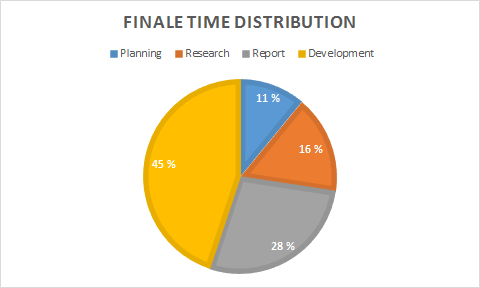
\includegraphics[width=0.9\textwidth]{fig/kake2.png}}
    \caption{Final time distribution}
    \label{fig:kake2}
  \end{figure}
\end{center}

\begin{center}
  \begin{figure}[h!]
    \makebox[\textwidth]{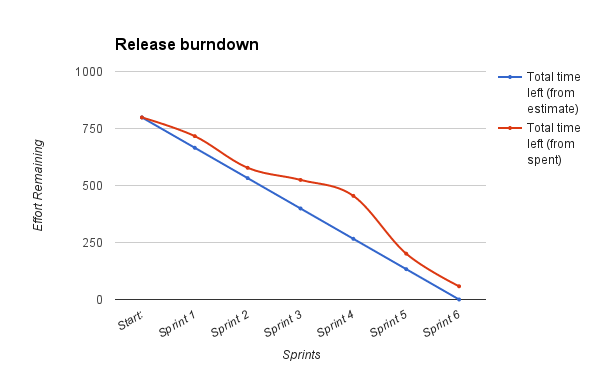
\includegraphics[width=\textwidth]{fig/burndown/releaseBurndown.png}}
    \caption{Overall burndown chart}
    \label{fig:release-burndown}
  \end{figure}
\end{center}

\section{Social and cooperational aspects}
\label{sec:Social_and_cooperation_aspects}

Group dynamic was rarely an issue. No social issues arose, and a nice work environment was upheld throughout the project. Eating lunch together, and taking breaks to talk about other things than the project made the days quite enjoyable. The social aspect helped throughout the project. It kept the morale of the group high, and promoted creativity. There were some minor arguments during the development phase. These were mainly due to different opinions on code principles, report structure and so forth. None of these arguments led to any anger or issues between anyone in the group, and were handled in a proper manner.

Cooperation worked out well throughout the project, both within the group, and with the customer and supervisor. It was easy to ask questions to other members, who were helpful if someone was stuck on a specific task or problem. Additionally, group meetings functioned as an arena where more complex tasks could be assessed by the whole group. All this made development more efficient, as it often prevented long periods of time being used on a specific problem. Meeting agendas were key when communicating with the customer and supervisor. The agendas provided a simple way of structuring each meeting, and they made sure nothing was forgotten or neglected.

The group also occasionally talked with other group's. The discussions were mainly about status on each group's project, and occasionally helping each other with report structure. The insight into other groups' work was helpful, as the group had someone to compare work with. This was sort of an additional safety net, to make sure no important parts of the project were neglected.

\section{Implementation}
\label{sec:Implementation}

Looking back at the group's initial expectations, compared to the challenges and complexities of the task known today, the group is very pleased with the result. What seemed like a somewhat straight forward implementation using existing libraries, turned into tough challenges and exploration.

It is worth mentioning that to the best of the group's knowledge, no other application exists that does what the group was asked to develop. The group did not manage to find a single multi-protocol brokering application supporting the WSN protocol. Additionally, general purpose clients were also very hard to find, thus resulting in the use of libraries to implement simple test clients during development. This created additional challenges, as best practices and documentation was hard to come across. Through much research, trial and error, the group eventually managed to overcome most of these challenges.

The group had to research, learn and implement several new patterns and best practices in order to develop a professional product. The steep learning curve served both as a source of frustration, as well as a source of motivation and reward. It is safe to say that the group members now have a much firmer grasp on what it takes to develop this kind of complex application. Although there are some areas of the implementation that have shortcomings, lack some unit tests, or other issues, the product as a whole works very well. The group is pleased with the degree of modularity, automation, and extendability it managed to implement.

The final system test showed that the group had met all the functional requirements. The shortcomings previously mentioned were uncovered or confirmed in the additional system tests. The main functional requirement results are listed in table \ref{table:system-testing-cases-fr1} through \ref{table:system-testing-cases-fr6}. As such, the group argues that the final outcome is a good product, that delivers as expected or better.
In depth explanations of the different challenges and shortcomings are described in subsequent sections below.

\subsection{Web technologies}
\label{subsec:Web_technologies}

Bootstrap and jQuery generally made it simpler and less time-consuming to build the administration interface. Bootstrap also made it simple to give the site a clean and intuitive design. All the requirements (see section \ref{sec:requirements_engineering-functional_requirements}) related to the administration interface were tested and met.

In retrospect, using WebSockets \cite{web-sockets} would have been a better approach for the administration interface. The system is now designed with AJAX for real-time update of content. This is not very scalable, and may result in high server load. Using WebSockets for this purpose would have proven much more efficient. Similar to the publish/subscribe pattern, WebSockets notify clients on a state change, instead of the clients constantly asking the server for the newest state. WebSockets would not make AJAX obsolete, but it would have been a better solution for serving true real-time update of content. AJAX would still have been used for making short-lived web service calls (e.g. HTTP DELETE requests).

\subsection{Broker}
\label{subsec:Implementation_broker}
Implementing the broker was a real challenge. Not only did the group have to figure out how to develop a working broker, but also to implement it in a way that followed the stated design and architecture goals. Questions like "How should messages be represented?", "How should topics and messages be connected?" and "How should messages be distributed?" were of paramount importance.

Much inspiration was gathered during the research phase, while investigating the Apollo broker. Several aspects of how it was designed became guidelines for how the group would implement the broker. There are vast differences of course, but some of the same patterns and techniques were used to achieve a robust implementation.

All in all the group is quite pleased with how the broker implementation turned out. It can consume messages very rapidly, and it instantly dispatches them as singular tasks in the core executor service. The executor in turn dynamically scales its number of concurrent threads to best suit the workload. This helps mitigate differences in how effective different protocols are, such that one resource heavy protocol does not cause starvation for another. In retrospect, there are ways it could have been improved of course. Allowing different priorities on message types, reuse of data structures for optimization, and a more elegant way of calling each protocol server's \verb!sendMessage()! method are some aspects.

Regardless, there is one high-level problem that still persists. The problem is related to translation between different protocols using vastly different representational structures. In the case of WSN, XML is used. A property in XML known as namespacing (discussed in the subsequent section) will cause translation problems with non-namespaced structures. In short, namespacing is used to allow multiple occurrences of elements with the same name. Without prior knowledge of what format the client is expecting, it seems (to the group) impossible to know which subscriber to send a non-namespaced message to. A message containing non-namespaced XML in an element called "result" will have to either be delivered to all subscribers regardless, or by retrieving schema definitions from all the clients to test which one matches the actual data. The latter would cause a huge performance hit, and might be impossible if schemas are not available. The same goes for namespaced topic expressions used in WSN. This problem will have to be adressed for all protocols that support some form of namespacing, when translating from non-namespaced protocols.

To summarize the group's thoughts on this particular challenge, it seems likely that this must be addressed by the operators of both the broker and the clients in use. In order to secure consistent behaviour which is predictable, some form of standard approach must be declared. Thus, the group leaves this question to system operators and their development teams, as they know their domain and usage pattern best.

\subsection{WSN}
\label{subsec:evaluation-implementation-wsn}

The WSN protocol was one of the core requirements of the system, as it is the NATO standard chosen for publish/subscribe protocols. The group was provided with the WS-Nu library, an implementation of the WSN protocol previously developed by students at NTNU. In addition to this library, attempts to find similar implementations were made. With the exception of modules built into commercial enterprise systems, the group did not find a single library other than WS-Nu.

Implementing the WSN protocol from scratch was out of the question, as the amount of time it would take far exceeded the time available. The findings in the prestudy showed that the WS-Nu library seemed well written, followed some familiar patterns and was not overly complex. As such, there was really no other option than to use the WS-Nu library.

One of the first challenges of implementing the WSN protocol was to get an overview of the WS-Nu implementation itself. It is a large project, that was probably developed over the course of a semester. It is also built around the fact that the WSN protocol is designed for use as a web service. All the different components of WS-Nu therefore act as web services. This meant that the group had to re-implement many of these components to allow interception and modification where needed. This was a daunting task, and took a lot of time to get right.

Nonetheless, this period of research, trial and error also provided some inspiration on how the group could solve other problems in the OKSE system. After some time, and a series of eureka moments, development progressed smoothly and quickly, until some shortcomings, faults and design issues appeared.

\subsubsection{Shortcomings and faults}
\label{subsec:evaluation-implementation-wsn-shortcomings_and_faults}

The first of the WS-Nu shortcomings was that the act of distributing messages to subscribers was implemented in a procedural and synchronous way. This meant that any subscriber that had lost its internet connection, or had a long latency, would cause the remaining subscribers to wait. A theoretical worst-case scenario can be illustrated as 100 subscribers, where the first 99 have lost their connection. With the default connection timeout of 15 seconds, this would accumulate to a total wait time of just under 25 minutes. A totally unacceptable bottleneck. The group circumvented this problem by assigning each message a slot in the brokers internal executor service, allowing large-scale concurrency.

Shortly thereafter, issues with a property of XML called namespaces were discovered. Namespaces are used to allow multiple elements in a document to contain the same element name. To prevent two systems creating and reading documents causing trouble for each other, namespaces are used to identify which domain the element name belongs to. The WS-Nu namespace context resolver produces duplicate namespace declarations in some cases. This is not something that will likely break any applications, as most parsers will just issue a warning if duplicate namespaces are encountered.

During the implementation of a specific type of WSN topic called a \verb!FullTopic!, issues with the expression validator were discovered. The groups additional system tests revealed that use of the \verb!*! wildcard operator in the expression failed to return what should have been valid subscribers. This flaw was discovered too late, and was in a complex evaluation part of the WS-Nu library. Hence, this flaw still persists in the OKSE system, when using WSN \verb!FullTopic! topics.

When a connection is made to send a message to a WSN subscriber, fixed content length is used until a certain message size is surpassed. This is defined internally in the Jetty HTTP client. The group discovered what seems to be a bug in the client, which causes a strange \verb!IllegalStateException!. This was discovered after the product was considered to be finished, and emergency debugging was started. The reason seems to be that the client does not properly handle the input stream of data properly. When buffering the entire stream and sending it as a single chunk of data, no errors occur. The group tested replacing the input stream with static data converted to a generic Java \verb!ByteArrayInputStream!. This was done to rule out the possibility that the fault lay in other parts of the system. Still, even after the change the problem persisted when the size threshold was surpassed. This reassured the group that it was indeed a bug in the Jetty HTTP client. A fix was quickly implemented to pre-buffer outgoing messages before they are sent, to prevent the failing Jetty chunked transfer encoding to occur. As it stands, the OKSE system fully supports chunked transfer-encoding on incoming requests, but does not use it on outgoing requests.

A final WSN specific issue was discovered, but after thoroughly reading the protocol documentation, the group agreed that this issue is a client standards compliance issue. Details on this peculiarity is found in additional system test STA.23 in table \ref{table:system_testing-additional_test_cases}.

Shortcomings aside, the group is pleased with how the re-implementation of WS-Nu and embedding into the OKSE message brokering system turned out. Worst-case performance bottleneck was reduced considerably, and some optimizations were performed along the way.
An overview of which test cases that produced unexpected results are found in appendix \ref{appendix-c:system_test_cases}.

\subsection{AMQP}
\label{subsec:Implementation_AMQP}

During the first iteration of AMQP implementation, some challenges were uncovered. The largest one was the handling of topic and queues. As a queue is a different concept compared to a topic, the implemented solution gave the user an option to choose which solution to use. Implementing Simple Authentication and Security Layer (SASL) support for authentication was another issue that proved difficult. The solution was to let the user choose whether or not to use it. The solution was not optimal, but works as expected.

Another challenge regarding the construction of outgoing AMQP messages, was to convert a Java object to a fixed size byte array. As AMQP is a byte level protocol, this had to be resolved. The solution was to as accurately as possible calculate the objects byte size. This was done using qualified guessing by looking at the different parts of the object. After a lot of testing, the final guess only missed with between 6-12 bytes. The final size of an object was found by trial and error. 

After the finalization of AMQP, the testing of the protocol implementation revealed to be more difficult than first thought. Finding applications that implements the 1.0 standard was difficult. FFI provided a version of NFFIPlayer (see section \ref{subsec:prestudies-existing_solutions-micro_wsn_and_nffiplayer}) with AMQP which implemented the 0.9.1 standard. However, due to the significant changes in the standard, it could not be used to any extent.

To be able to test the implementation properly, a functioning implementation was required. Two AMQP 1.0 Java implementations were found, and simple scripts were written to test both send and receive functionality. As there was a limited amount of free/open implementations, the group ended up using one open source solution from Apache Qpid (not proton) \cite{apache-qpid} and one commercial from SwiftMQ \cite{swift-mq}. By using these implementations, the basis for stating the correctness of the implementation and the quality of the product was solid. The final test results are reflected in table \ref{table:system-testing-cases-fr11-13}. All of the tests regarding AMQP passed. As the AMQP implementation was quite a lot smaller than WSN, it was easier to test.
